\subsubsection{MIPS Pipelining}

In simple words, the Instruction Pipelining (or Pipelining) is a technique for implementing instruction-level parallelism within a single processor. Pipelining attempts to keep every part of the processor busy with some instruction by dividing incoming instructions into a series of sequential steps (the eponymous \dquotes{pipeline}) performed by different processor units with different parts of instructions processed in parallel.

\highspace
\begin{definitionbox}[: Pipelining]
    \indexdefinition{Pipelining} is a performance optimization technique based on the \textbf{overlap} of the execution of multiple instructions deriving from a sequential execution flow.
\end{definitionbox}

\noindent
Pipelining exploits the \textbf{parallelism among instructions in a sequential instruction stream}.

\begin{flushleft}
    \textcolor{Red2}{\faIcon[regular]{star} \textbf{Basic idea}}
\end{flushleft}
The execution of an \textbf{instruction is divided into different phases} (called \indexdefinition{pipelines stages}), requiring a fraction of the time necessary to complete the instruction. These stages are connected one to the next to form the pipeline:
\begin{enumerate}
    \item Instructions enter the pipeline at one end;
    \item Progress through the stages;
    \item And exit from the other end.
\end{enumerate}
As in the assembly line.

\begin{flushleft}
    \textcolor{Green3}{\faIcon{check} \textbf{Advantage}}
\end{flushleft}
The \textbf{Pipelining is transparent for the programmer}. To understand what it means, let's make an example.

\begin{examplebox}
    Image a car assembly line (e.g. Ferrari). A new car exits from the Ferrari assembly line in the time necessary to complete one of the phases. The pipelining technique doesn't reduce the time required to complete a car (the \textbf{latency}), BUT increases the number of vehicles produced per time unit (the \textbf{throughput}) and the frequency to complete cars.
\end{examplebox}

\newpage

\begin{examplebox}
    Image a sequential laundry jobs over time:\cite{pipelining-slides}
    \begin{center}
        \centering
        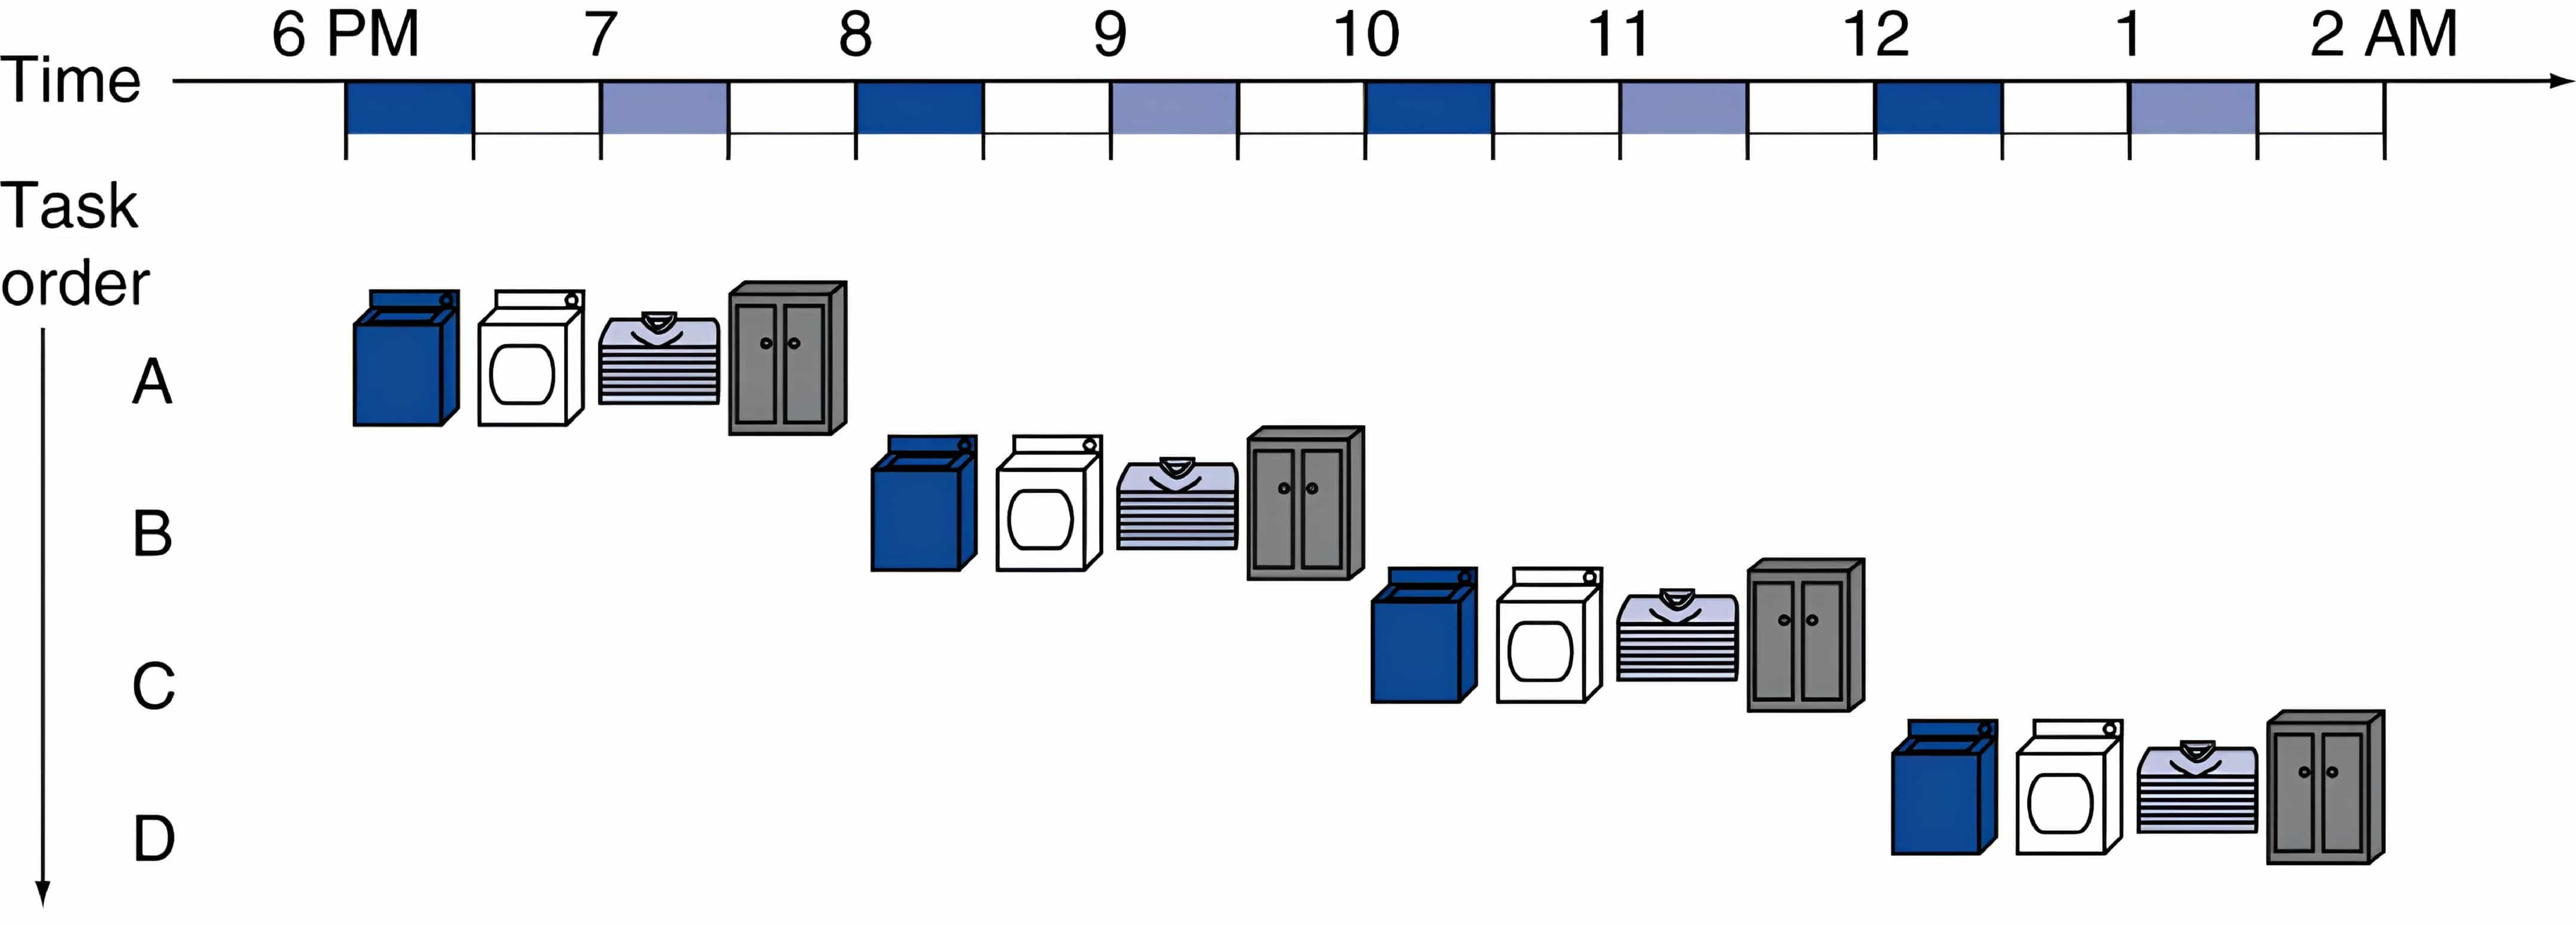
\includegraphics[width=.9\textwidth]{img/pipelining-example-1.pdf}
    \end{center}
    The pipelined laundry. Overlapping execution of stages to improve throughput (number of jobs executed per hour):\cite{pipelining-slides}
    \begin{center}
        \centering
        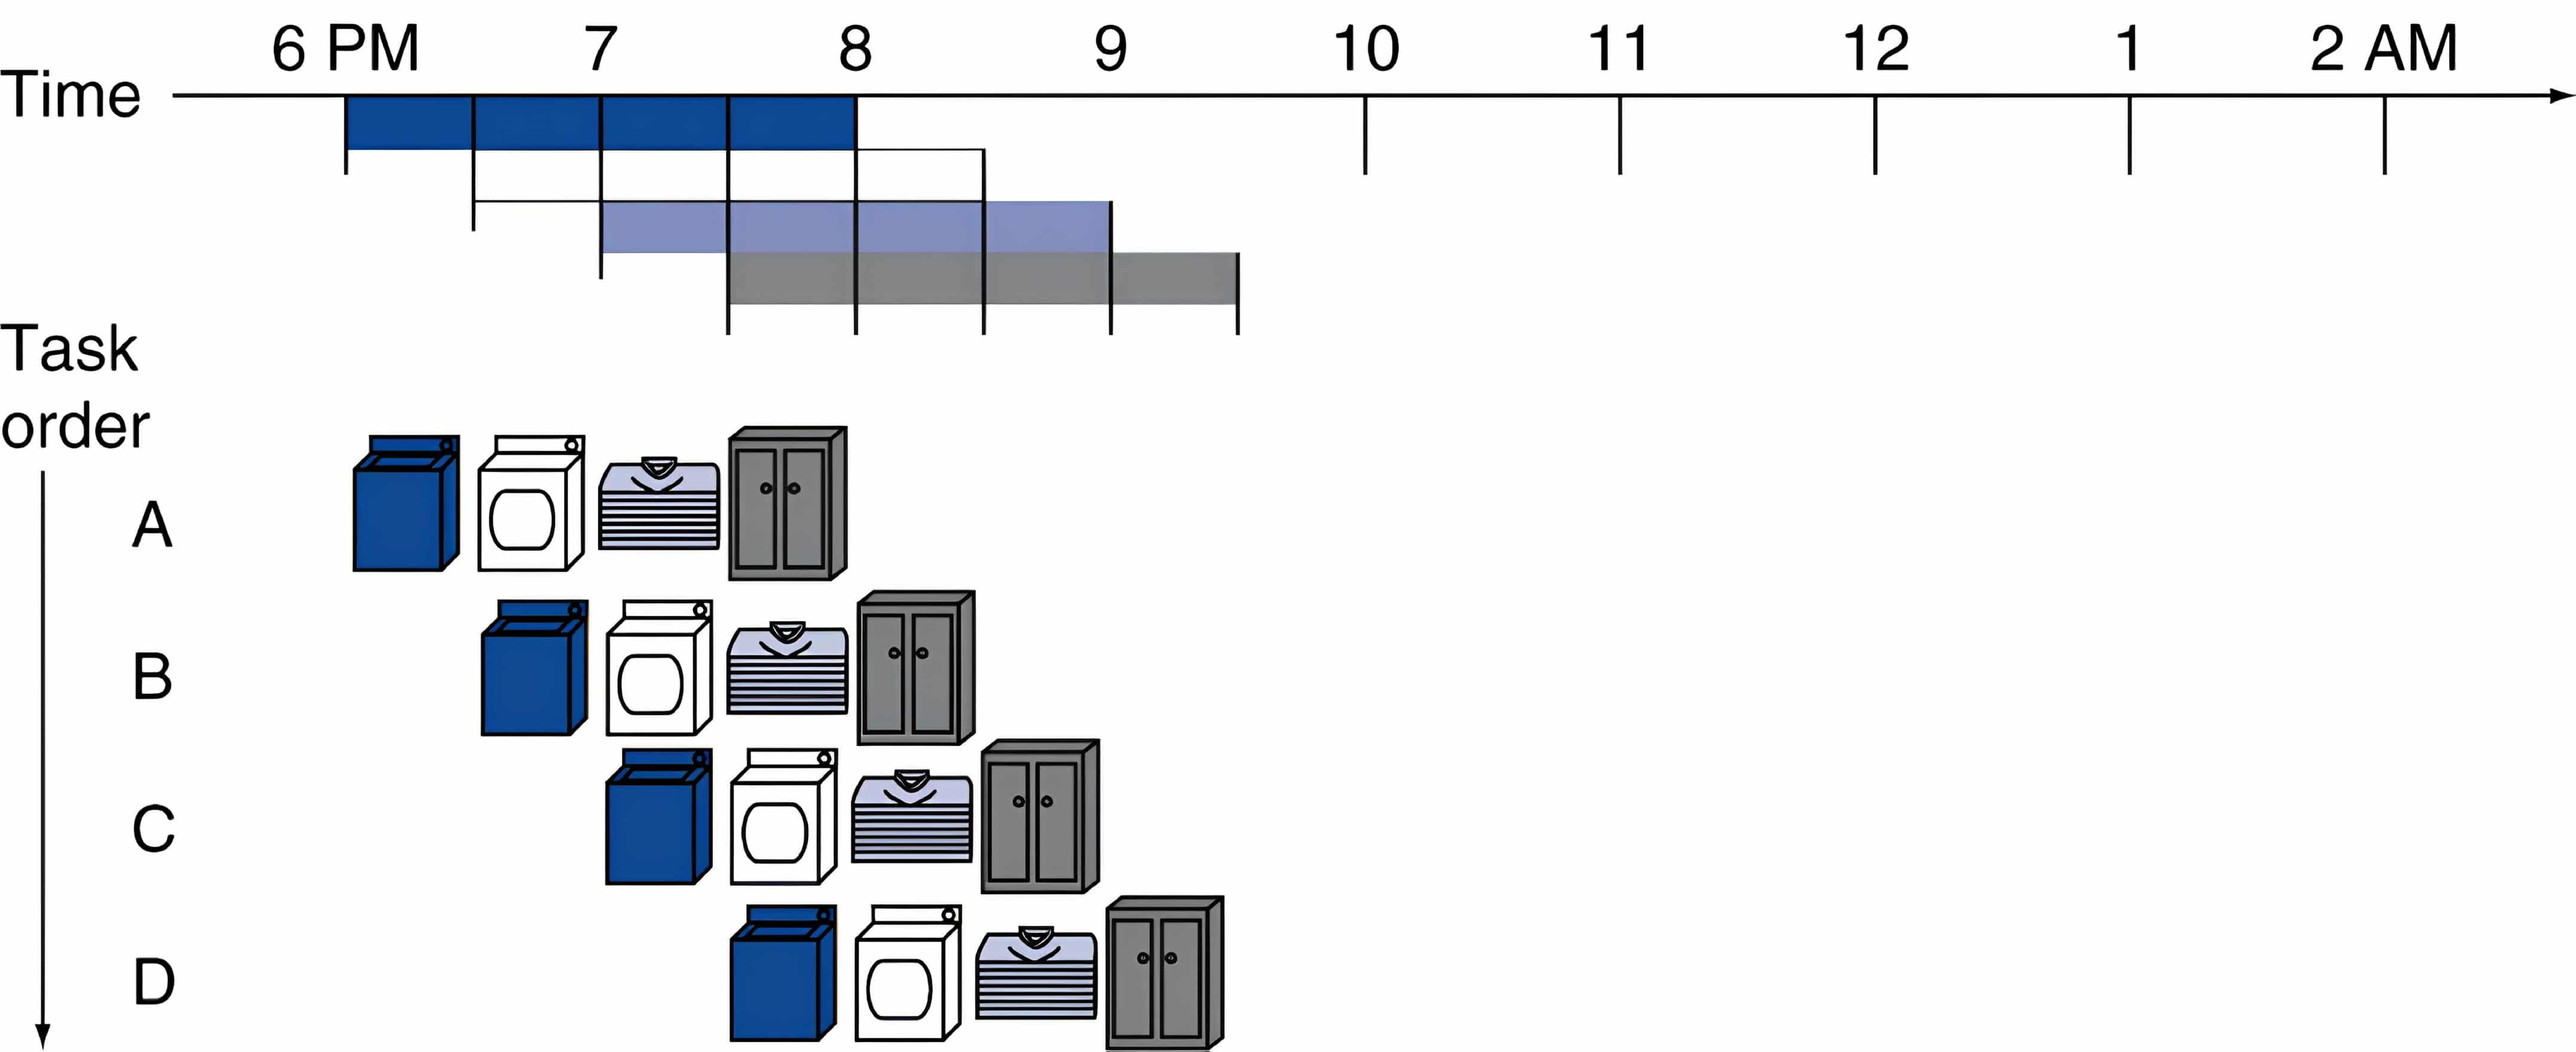
\includegraphics[width=.9\textwidth]{img/pipelining-example-2.pdf}
    \end{center}
\end{examplebox}

\noindent
As introduced in the previous example, sequential execution is slower than pipelining. The following figure shows the difference (in terms of clock cycles) between sequential and pipelining.
\begin{figure}[!htp]
    \centering
    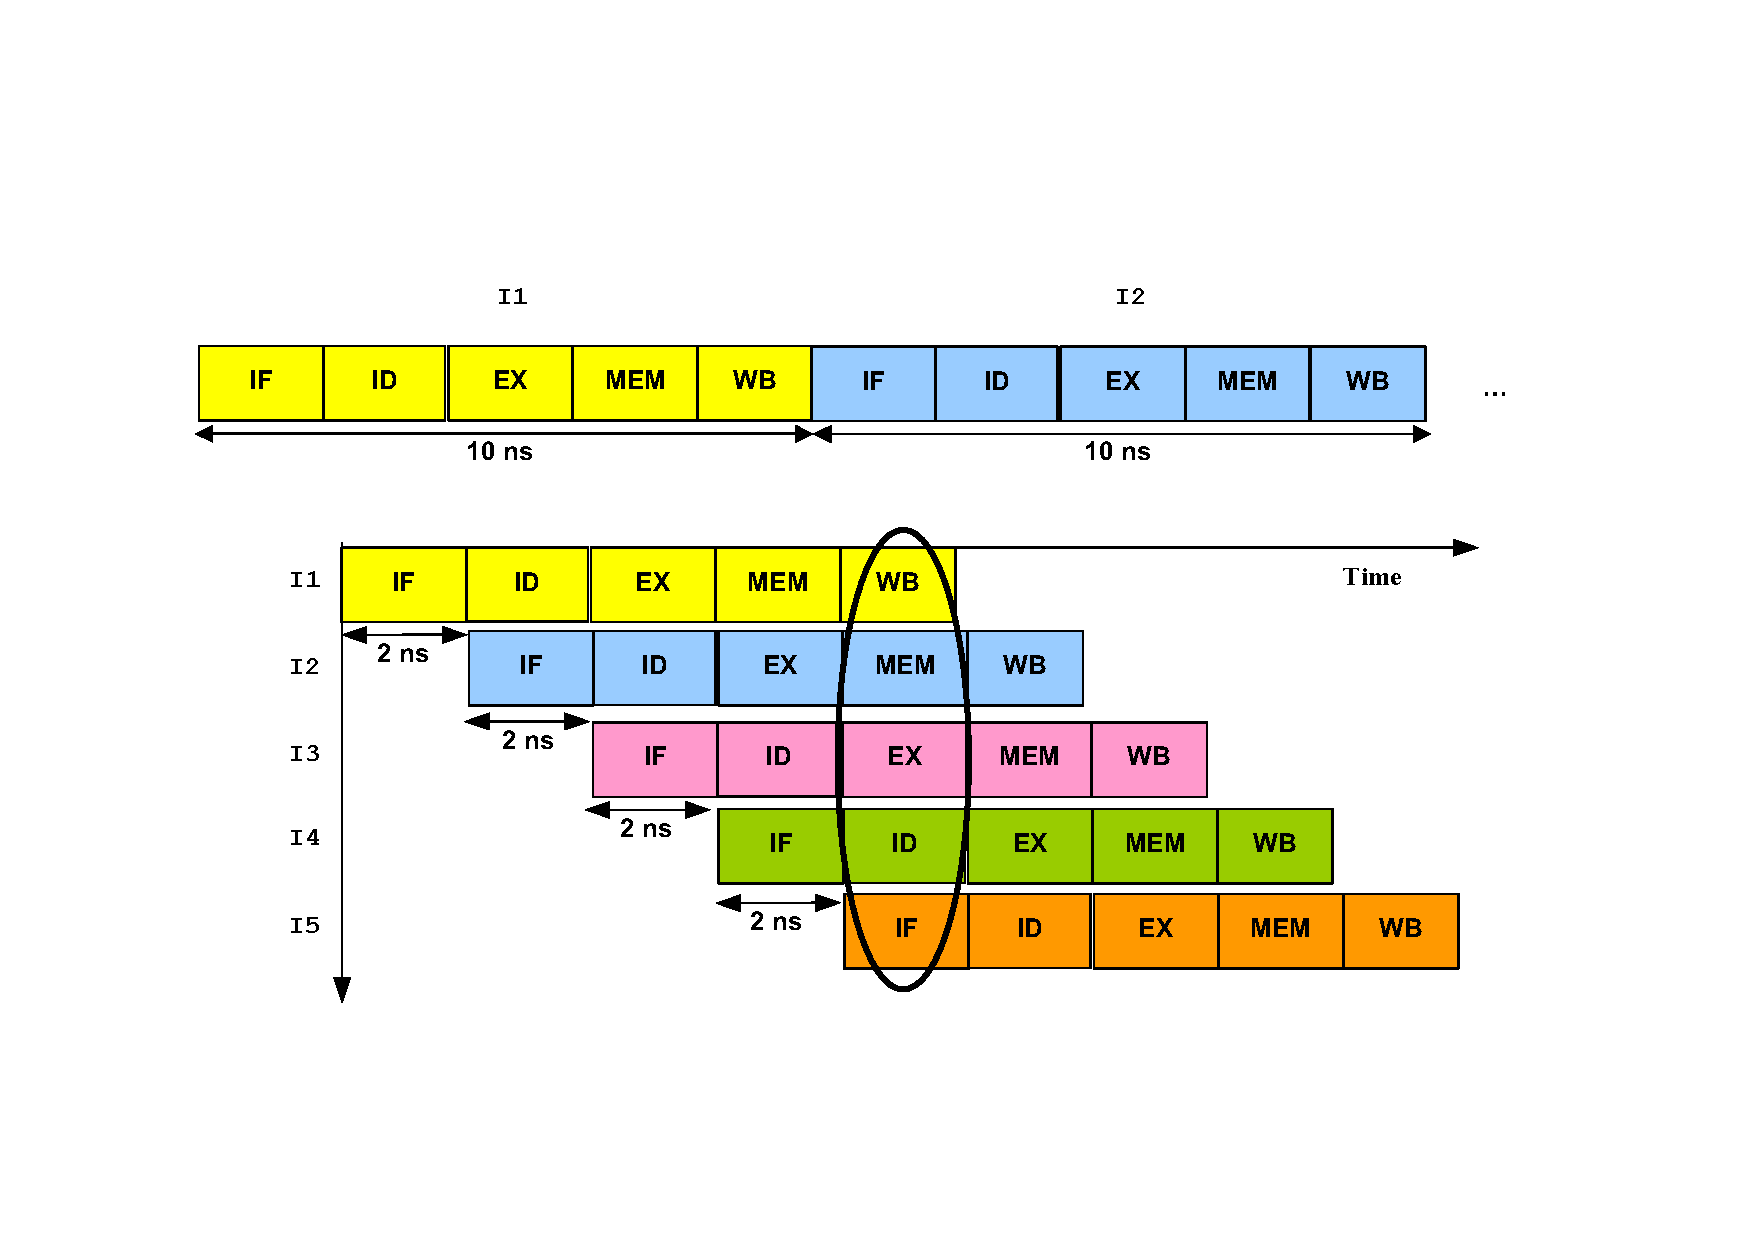
\includegraphics[width=\textwidth]{img/sequential-vs-pipelining-1.pdf}
    \caption{Sequential vs Pipelining.\cite{pipelining-slides}}
    \label{fig: sequential vs pipelining}
\end{figure}

\newpage

\noindent
The time to advance the instruction of one stage in the pipeline corresponds to a clock cycle. So the total cost is: 9 clock cycles.

\highspace
It's obvious that the \textbf{pipeline stages must be synchronized}: the duration of a clock cycle is defined by the time required by the slower stage in the pipeline (i.e. 2 ns). The \textbf{main goal} is to \textbf{balance the length of each pipeline stage}. If the stages are perfectly balanced, the \textbf{ideal speedup} due to pipelining is equal to the number of pipeline stages.

\begin{definitionbox}[: ideal speedup]
    The \indexdefinition{ideal speedup} must be the \textbf{same value of the pipeline stages}.
\end{definitionbox}

\highspace
Look again at Figure~\ref{fig: sequential vs pipelining}. The sequential and pipelining cases consist of 5 instructions, each of which is divided into 5 low-level instructions of 2 ns each.
\begin{itemize}
    \item The \textbf{latency} (total execution time) of each instruction is not varied, it's always 10 ns.
    \begin{definitionbox}[: latency]
        The \indexdefinition{latency} is the execution time of a single instruction.
    \end{definitionbox}

    \item The \textbf{throughput} (number of low-level instructions completed in the time unit) is improved:
    \begin{itemize}
        \item Sequential: 5 instructions in 50 ns (1 instruction per 10 ns, $50 \div 5 = 10$)
        \item Pipelining: 5 instruction in 18 ns (1 instruction per 3.6 ns, $18 \div 5 = 3.6$)
    \end{itemize}
    \begin{definitionbox}[: throughput]
        The \indexdefinition{throughput} is the number of instructions completed per unit of time.
    \end{definitionbox}
\end{itemize}

\newpage

\begin{center}
    \large
    \textcolor{Red3}{\textbf{Pipeline Execution of MIPS Instructions}}
\end{center}
On page~\pageref{Execution (EX) details} we discussed some MIPS instructions to understand how the MIPS architecture works. The aim of the following pages is to understand \textbf{how MIPS works in a pipelined execution}.

\highspace
We want to perform the following assembly lines:
\lstinputlisting[language=misc]{code/mips-pipelining/sequential-vs-pipelining.s}
\begin{figure}[!htp]
    \centering
    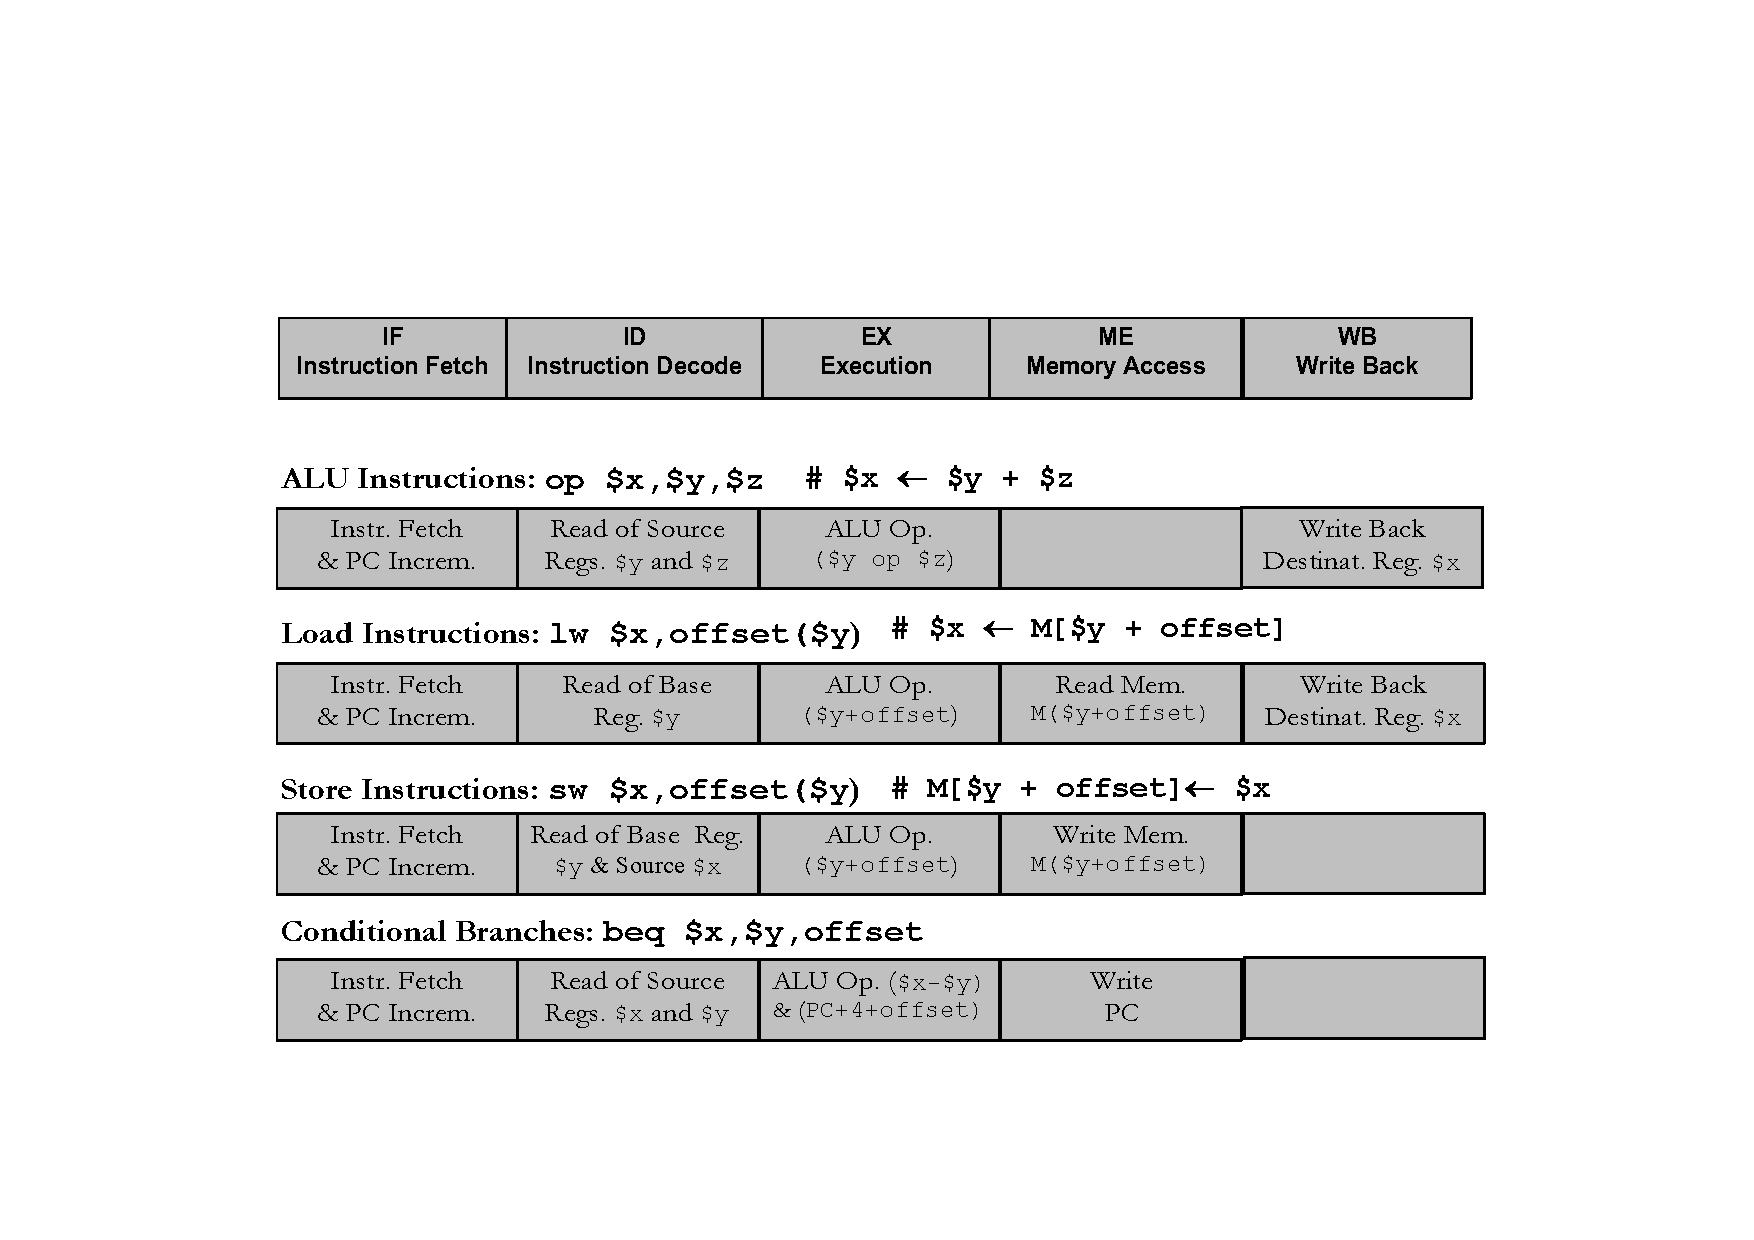
\includegraphics[width=\textwidth]{img/sequential-vs-pipelining-2.pdf}
    \caption{Pipeline Execution of MIPS Instructions.\cite{pipelining-slides}}
\end{figure}

\newpage

\begin{center}
    \textcolor{Red3}{\textbf{Resources used during the pipeline execution}}
\end{center}
\begin{figure}[!htp]
    \centering
    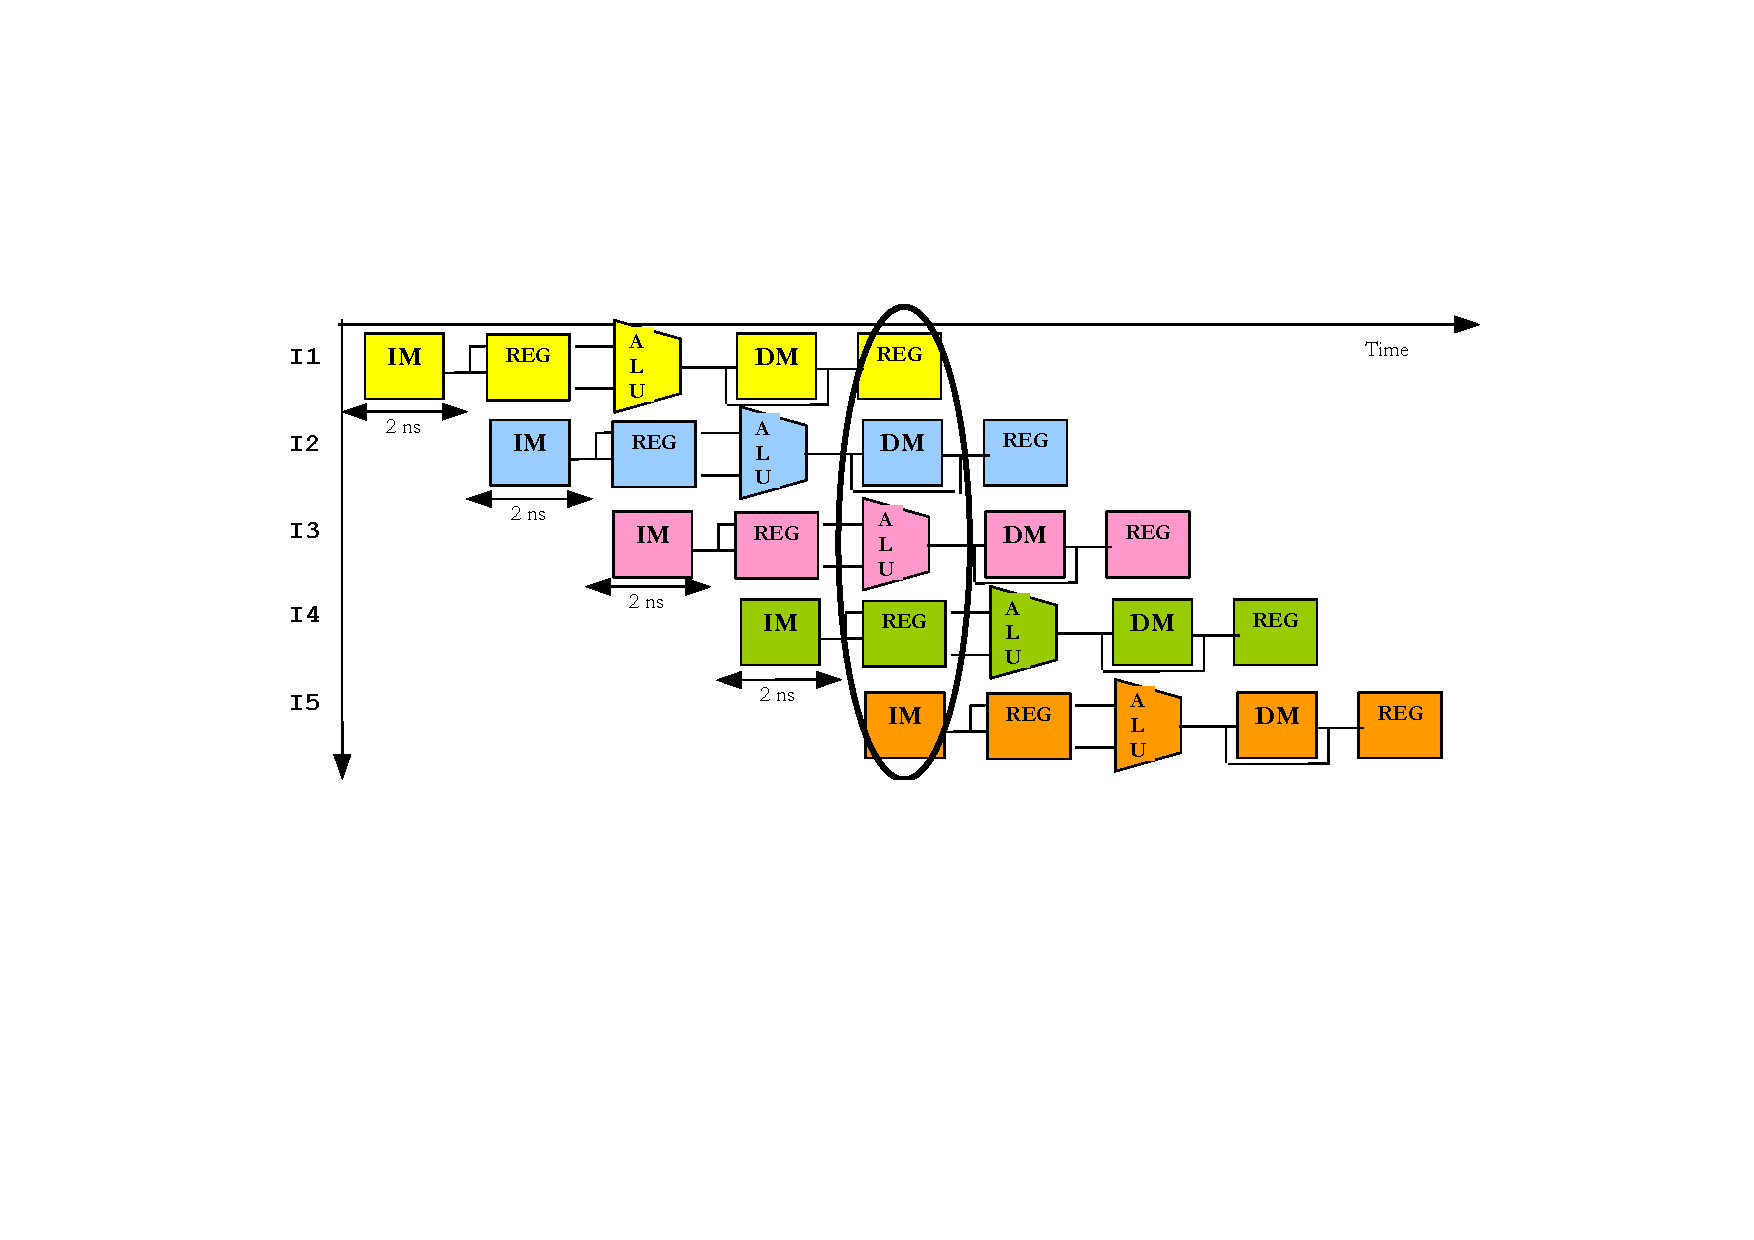
\includegraphics[width=\textwidth]{img/sequential-vs-pipelining-3.pdf}
    \caption{Resources used during the pipeline execution (IM is Instruction Memory, REG is Register File and DM is Data Memory).\cite{pipelining-slides}}
\end{figure}

\newpage

\begin{center}
    \large
    \textcolor{Red3}{\textbf{Implementation of MIPS pipeline}}
\end{center}
The division of the execution of each instruction in $n$ stages implies that in each clock cycle, there are $n$ instructions for execution. That means the CPU must have $n$ modules corresponding to $n$ execution stages. Therefore, to do pipelining, we need \indexdefinition{pipeline registers} \textbf{to separate the different stages}.

\highspace
In the following figure, we can see how the pipeline registers are implemented. Between each phase of execution of MIPS instructions (details on page \pageref{Phases of execution of MIPS Instructions}), there is a pipeline register holding the result of the instruction.
\begin{figure}[!htp]
    \centering
    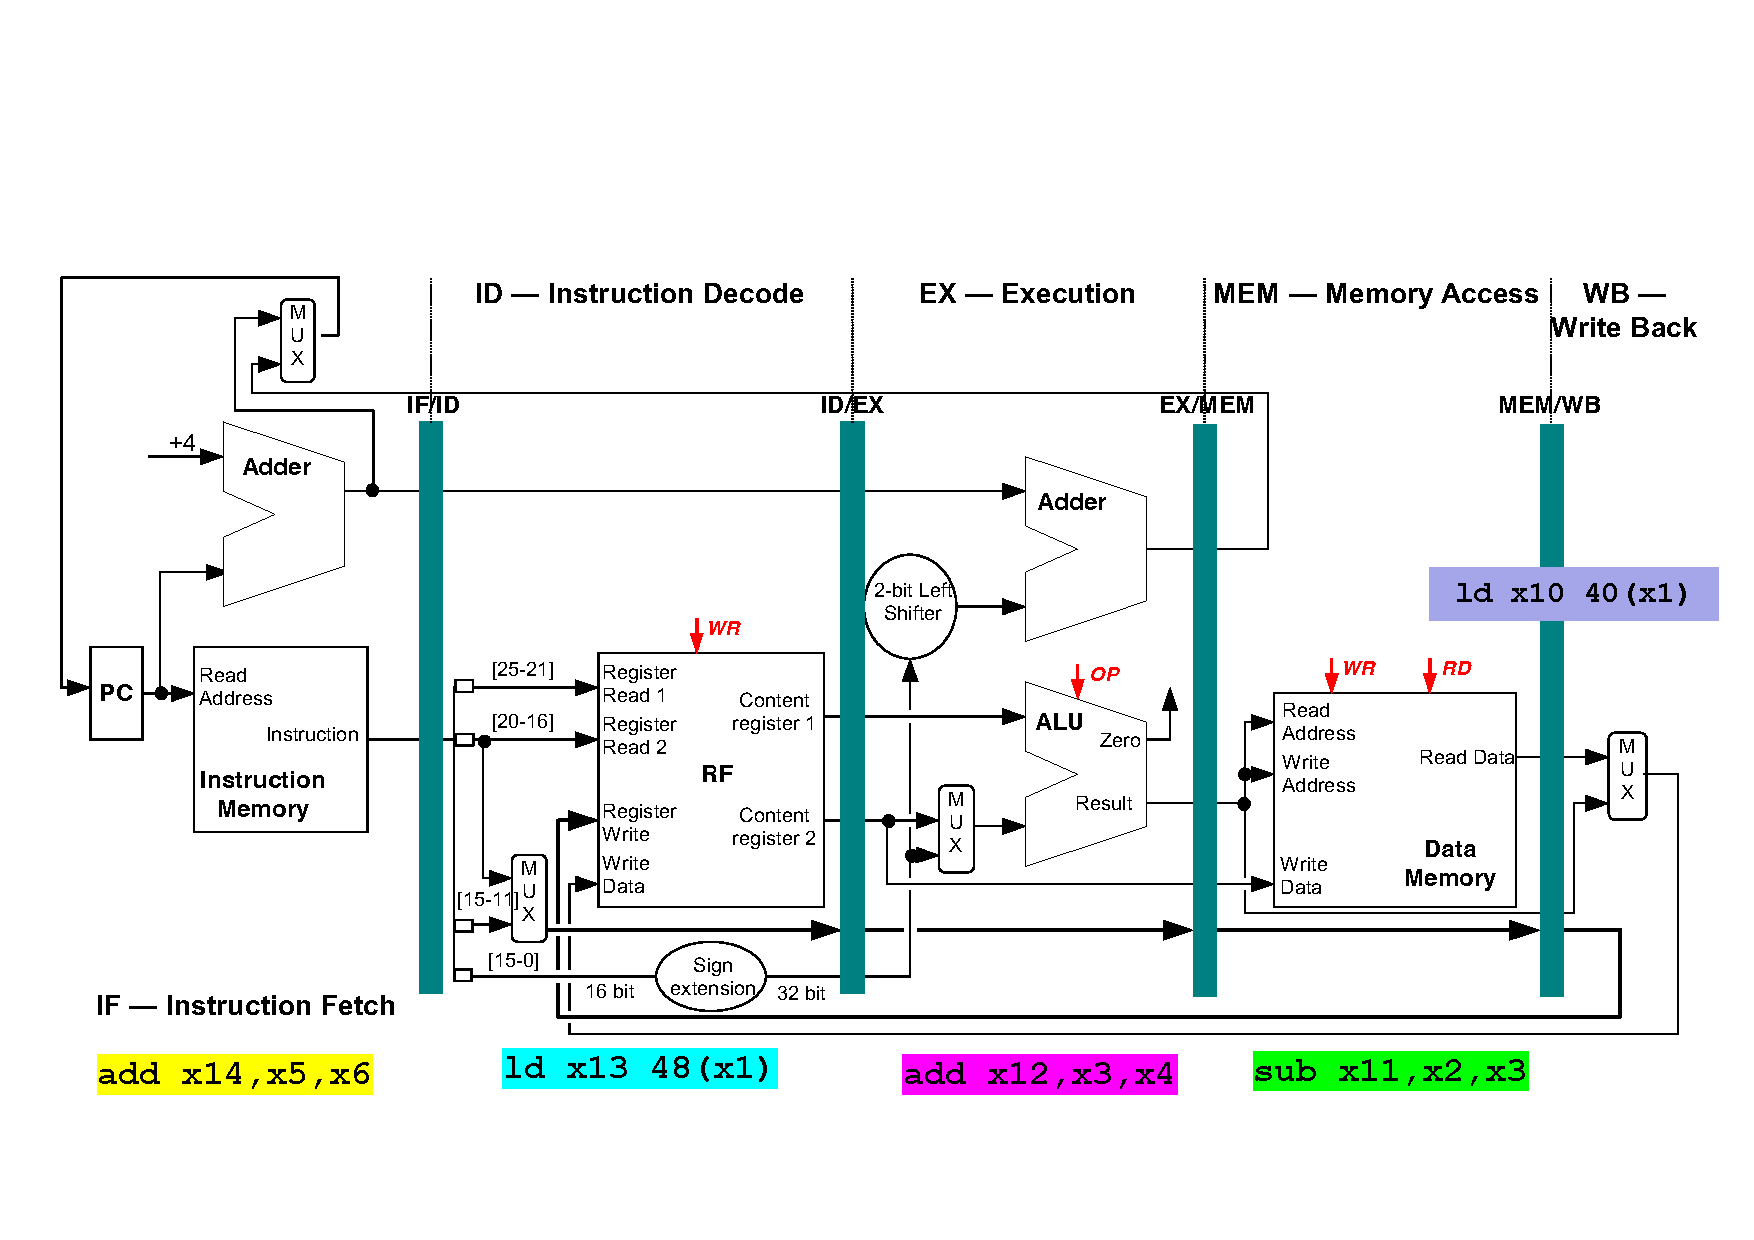
\includegraphics[width=\textwidth]{img/pipeline-registers-1.pdf}
    \caption{MIPS pipeline implementation.\cite{pipelining-slides}}
\end{figure}

\noindent
\underline{Note}: \textbf{the data stored in the interstage registers correspond (obviously) to different instructions}.

\newpage

\noindent
Finally, in the following figure we can see the timeline implementation of the pipeline registers. But there are two basic assumptions to make:
\begin{enumerate}
    \item There are no data dependencies between instructions. If there were, an instruction could read a register with an unknown value (Pipeline Hazard, page~\pageref{subsubsection: The problem of Pipeline Hazards}).

    \item There are no branch/jump instructions.
\end{enumerate}
\begin{figure}[!htp]
    \centering
    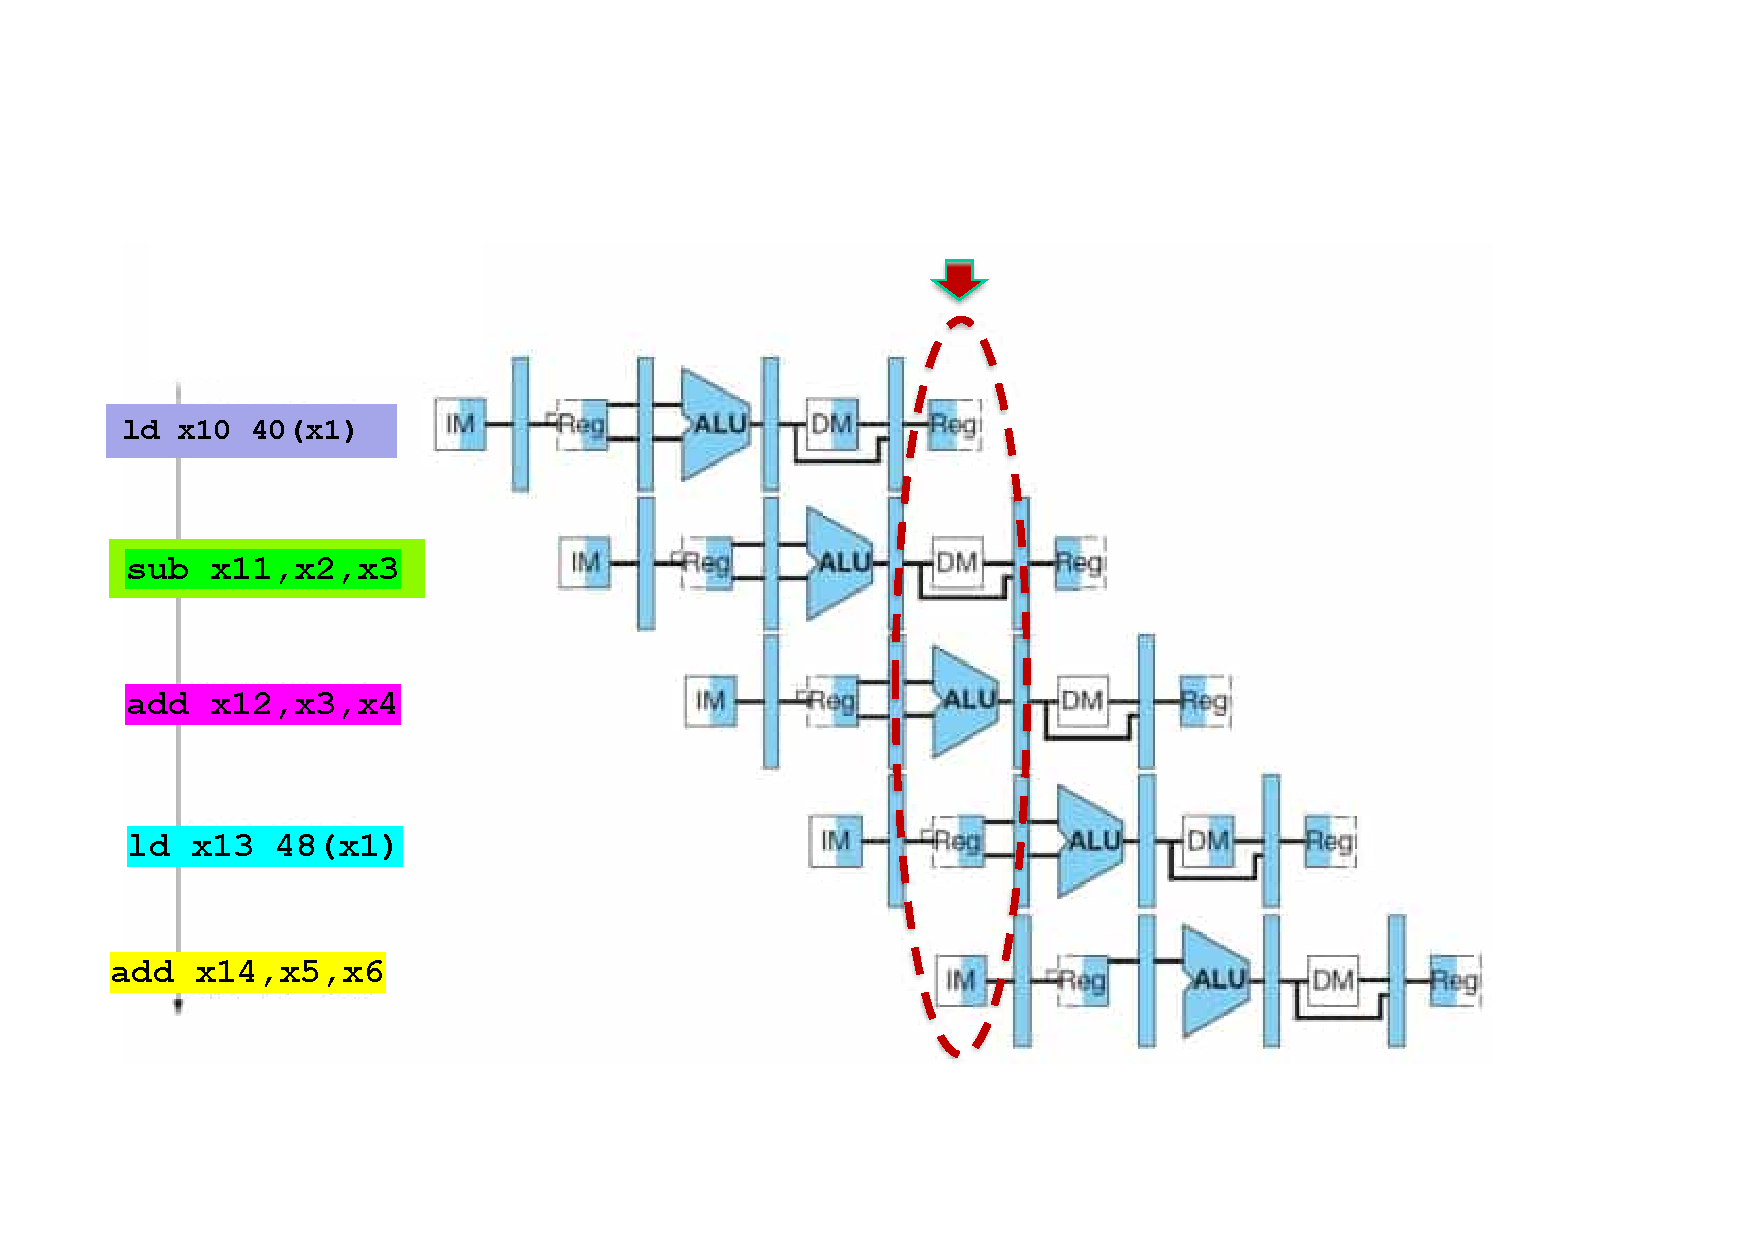
\includegraphics[width=\textwidth]{img/pipeline-registers-2.pdf}
    \caption{Timeline of MIPS pipeline implementation.\cite{pipelining-slides}}
\end{figure}